\documentclass[border=10pt]{standalone}
\usepackage{pgfplots}
\usepgfplotslibrary{colormaps}
\pgfplotsset{compat=1.18}

\begin{document}
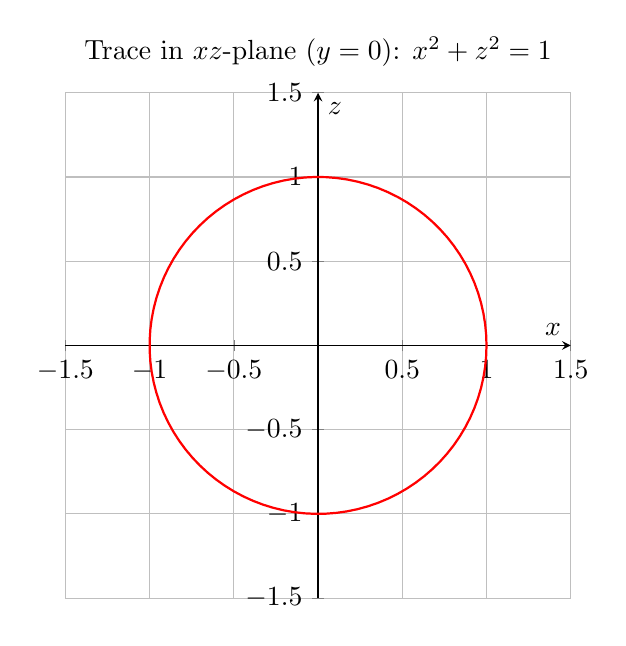
\begin{tikzpicture}
\begin{axis}[
    width=10cm,
    height=8cm,
    xlabel=$x$,
    ylabel=$z$,
    title={Trace in $xz$-plane ($y=0$): $x^2 + z^2 = 1$},
    axis lines=middle,
    xmin=-1.5, xmax=1.5,
    ymin=-1.5, ymax=1.5,
    axis equal image,
    grid=major,
    samples=100,
    domain=0:360,
]
\addplot+[mark=none, thick, red] ({cos(x)}, {sin(x)});
\end{axis}
\end{tikzpicture}
\end{document}
